\begin{flushright} {\tiny {\color{gray} python\_codes/fieldstone\_100/text.tex}} \end{flushright}

\lstinputlisting[language=bash,basicstyle=\small]{python_codes/fieldstone_100/keywords}

\begin{center}
Code at \url{https://github.com/cedrict/fieldstone/tree/master/python_codes/fieldstone_100}
\end{center}

\par\noindent\rule{\textwidth}{0.4pt}

{\sl This fieldstone was developed in collaboration with B. Root}. \index{contributors}{B. Root}

\par\noindent\rule{\textwidth}{0.4pt}
%%%%%%%%%%%%%%%%%%%%%%%%%%%%%%%%%%%%%%%%%%%%%%%%%%%%%%%%%%%%%%%%%%%%%%%%%%%%%%%%%%%%%%%%%%%%%%

Very high resolution topography datasets of Mars are available at 
\url{https://astrogeology.usgs.gov/search/details/Mars/GlobalSurveyor/MOLA/Mars_MGS_MOLA_DEM_mosaic_global_463m/cub}.
However the data format is not very convenient so Bart Root 
helped me out and exported the data to ascii format.

The file {\filenamefont MOLA\_1deg.txt} counts 64,800 lines, 
i.e. 360x180 points. Longitude values range from  
0.5 to 359.5 and latitudes from -89.5 to +89.5. 

The file {\filenamefont MOLA\_0.5deg.txt} counts 4 times as many lines, 
i.e. 720x360 points. Longitude values range from  
0.25 to 359.75 and latitudes from -89.75 to +89.75. 




We follow a similar approach as in \stone 97 and use the data to produce 
two vtu files, one on a 2D plane, one on a 3D sphere:

\begin{center}
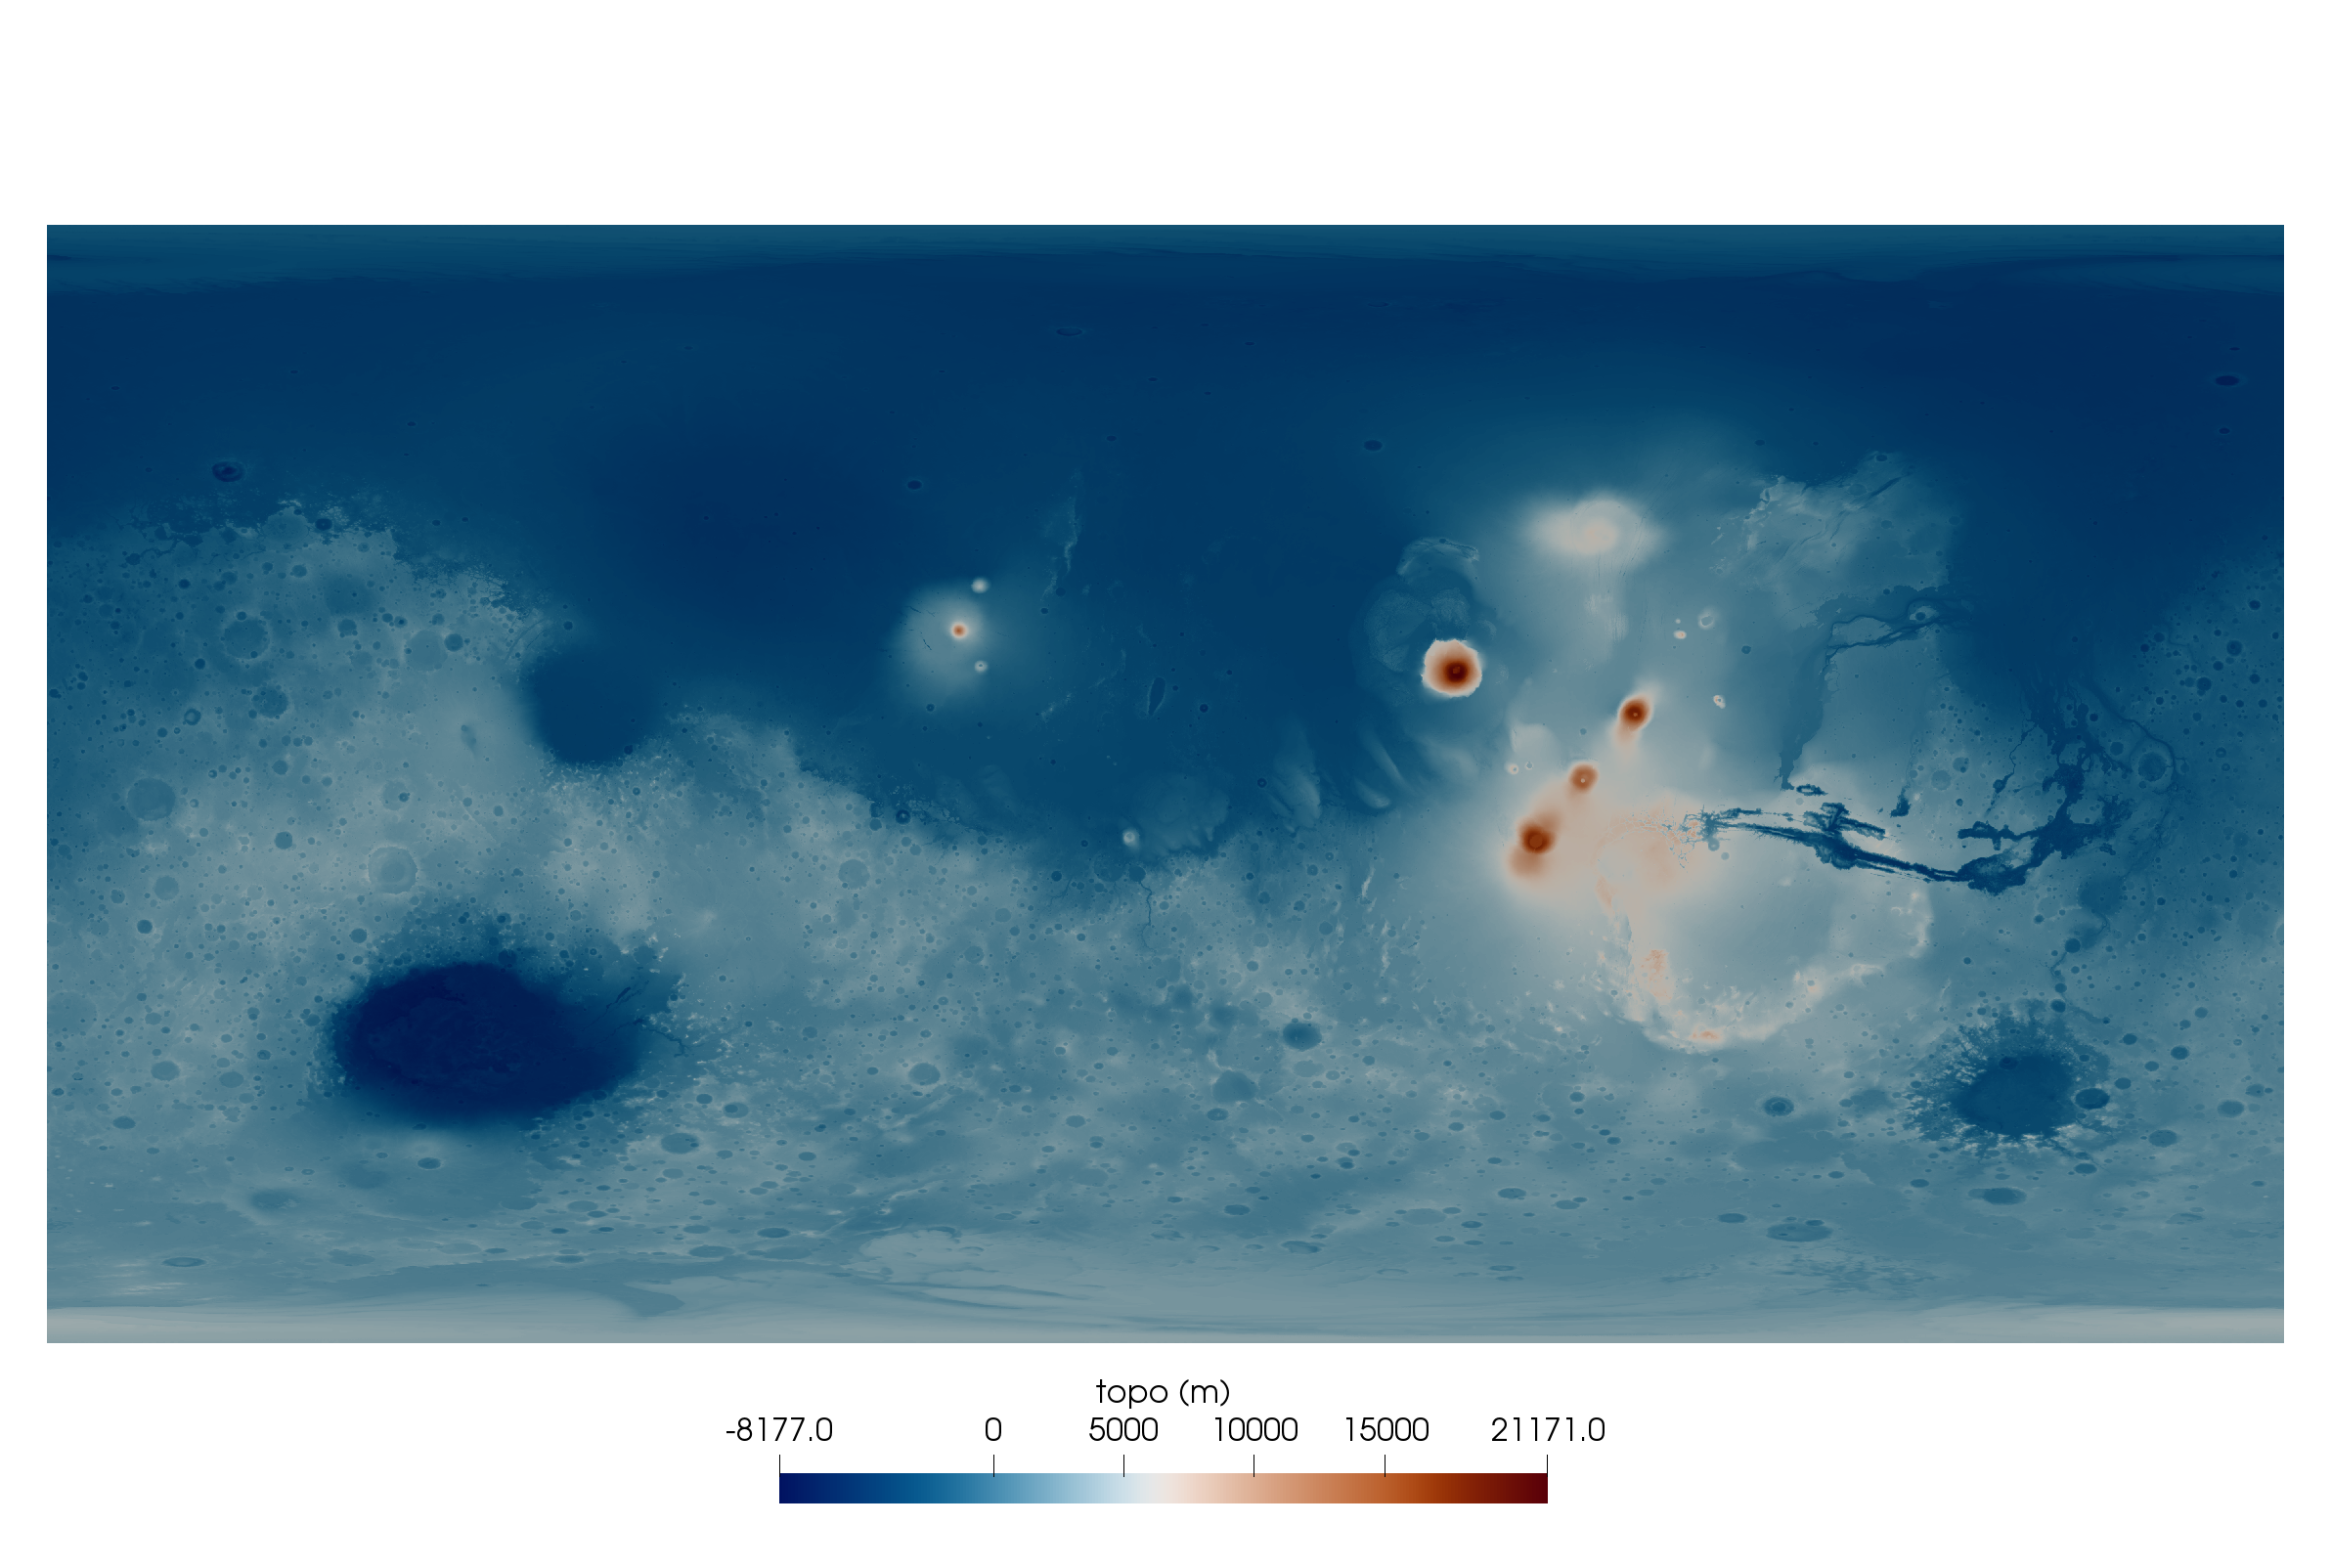
\includegraphics[width=15cm]{python_codes/fieldstone_100/images/topo2D_a}\\
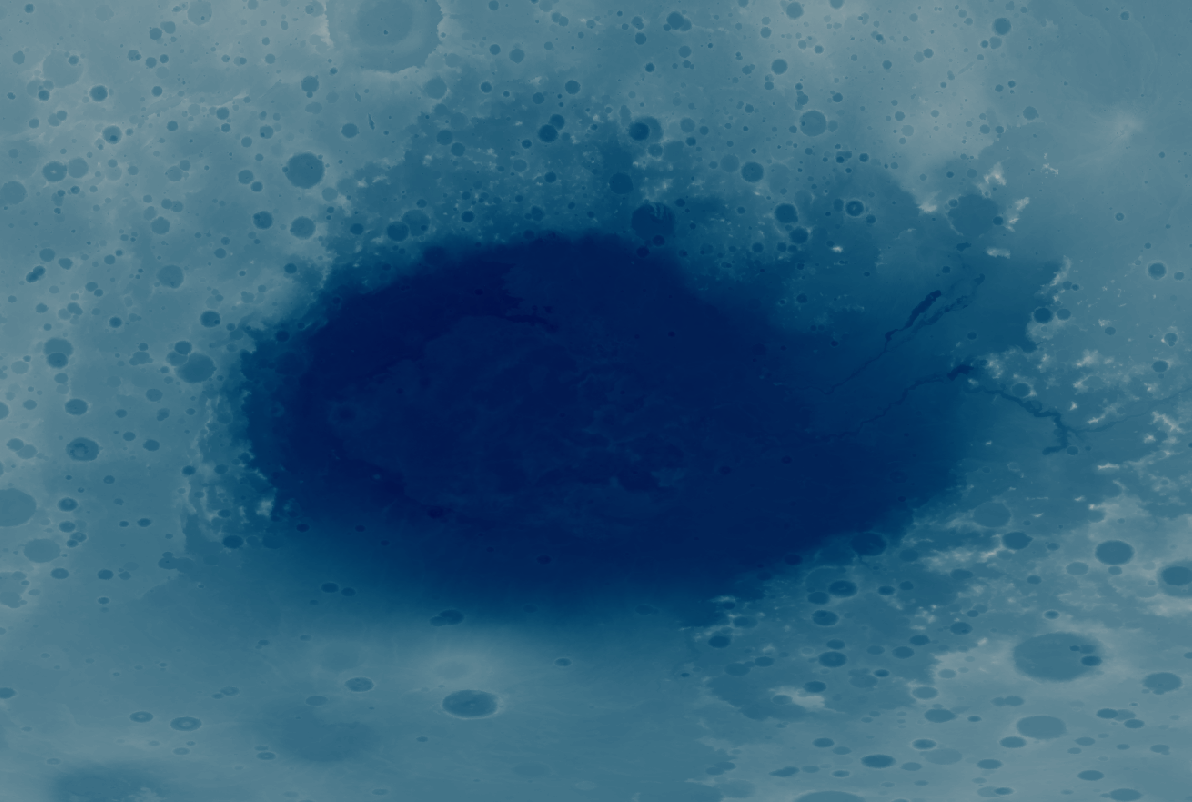
\includegraphics[width=5cm]{python_codes/fieldstone_100/images/topo2D_b}
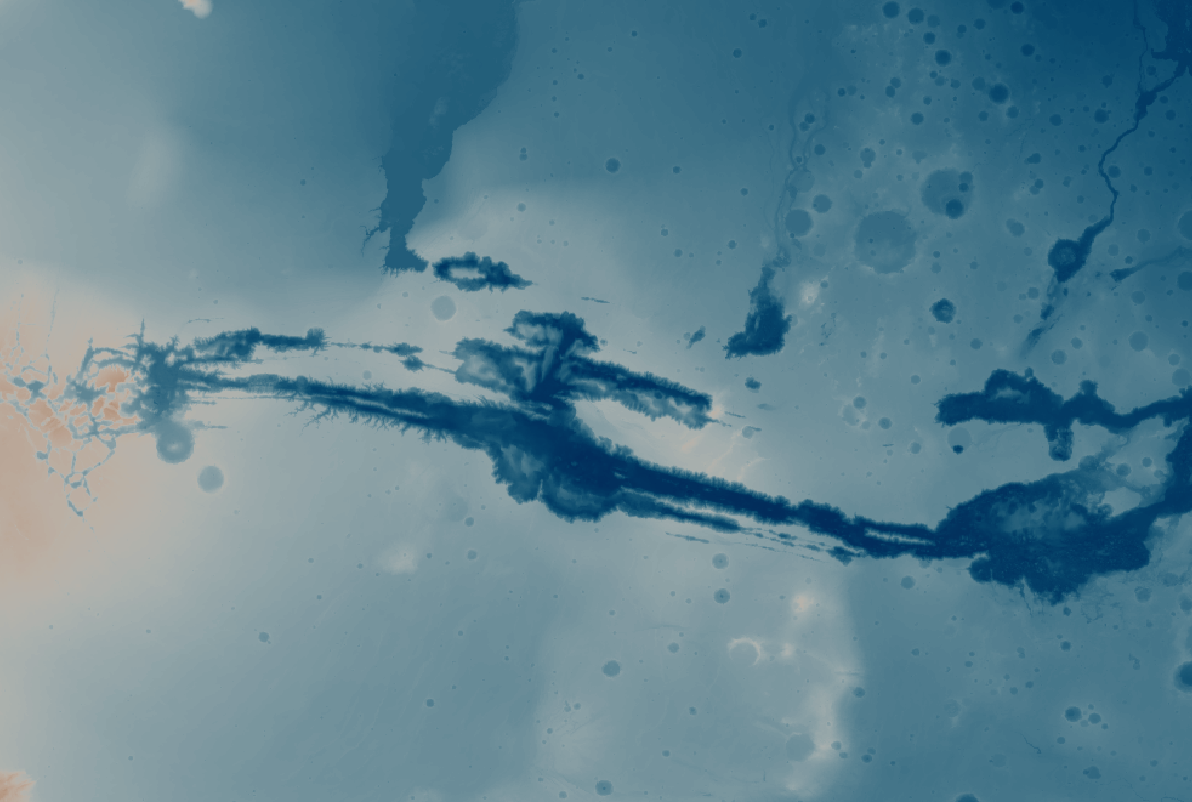
\includegraphics[width=5cm]{python_codes/fieldstone_100/images/topo2D_c}
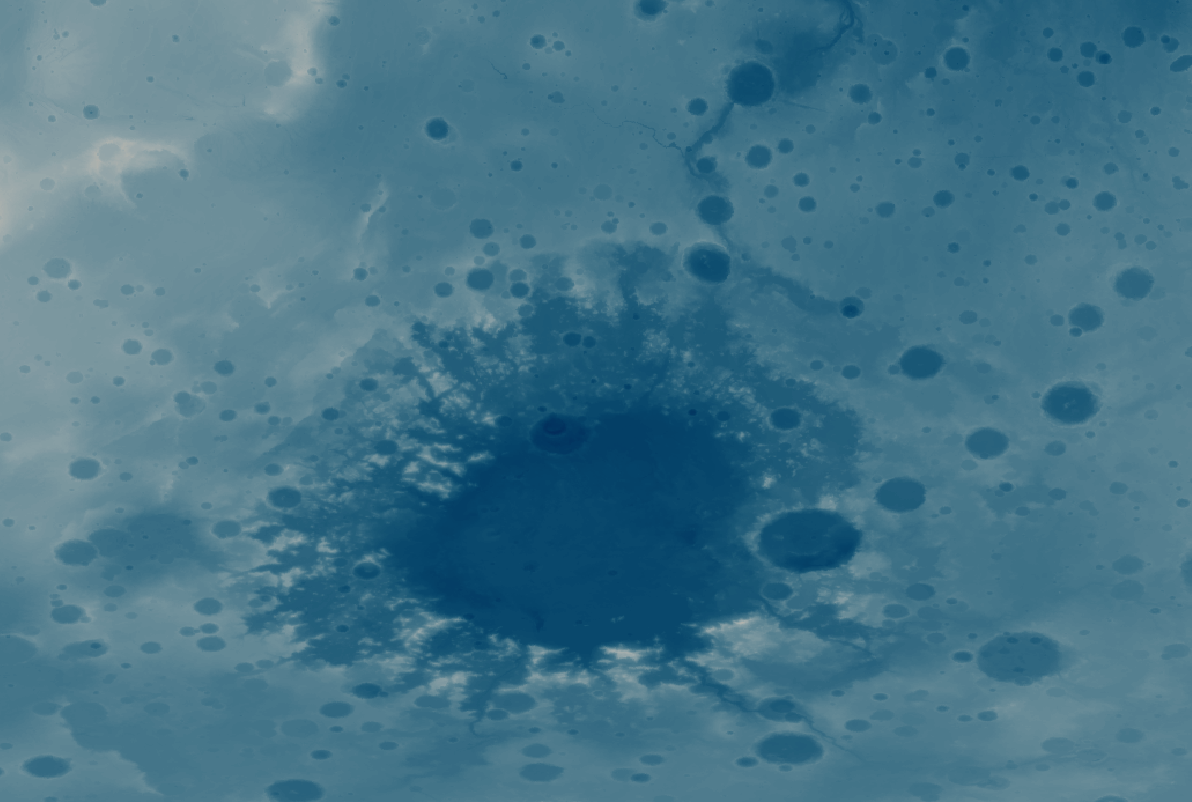
\includegraphics[width=5cm]{python_codes/fieldstone_100/images/topo2D_d}\\
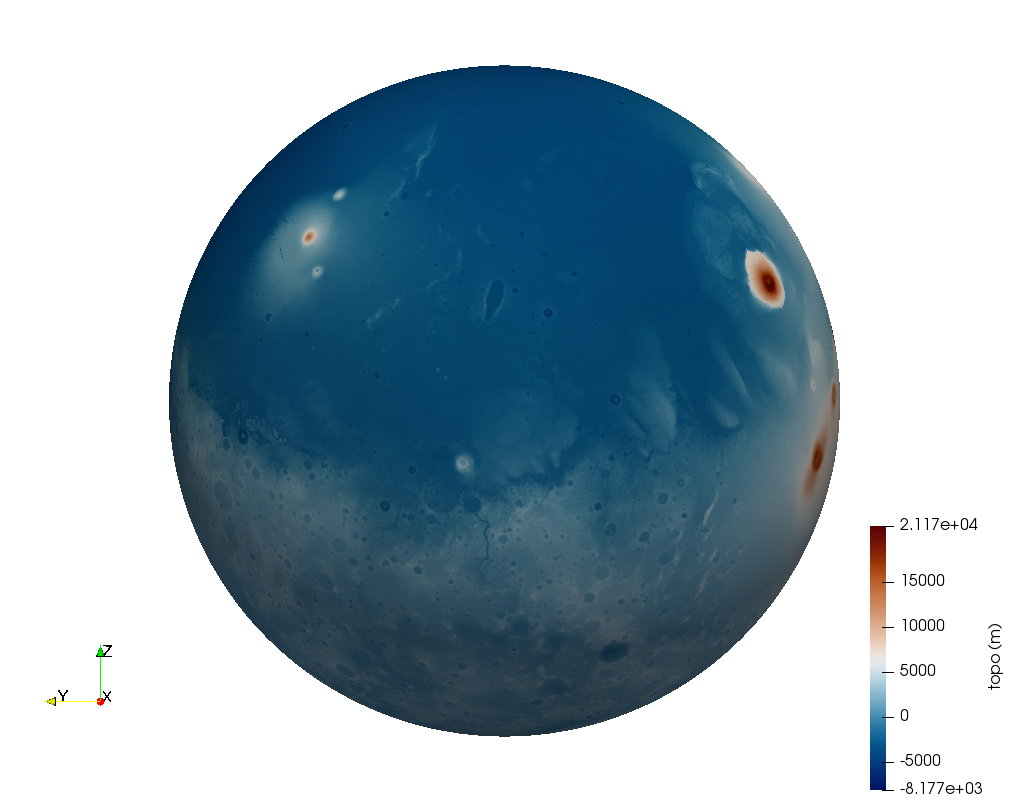
\includegraphics[width=5cm]{python_codes/fieldstone_100/images/topo3D_1}
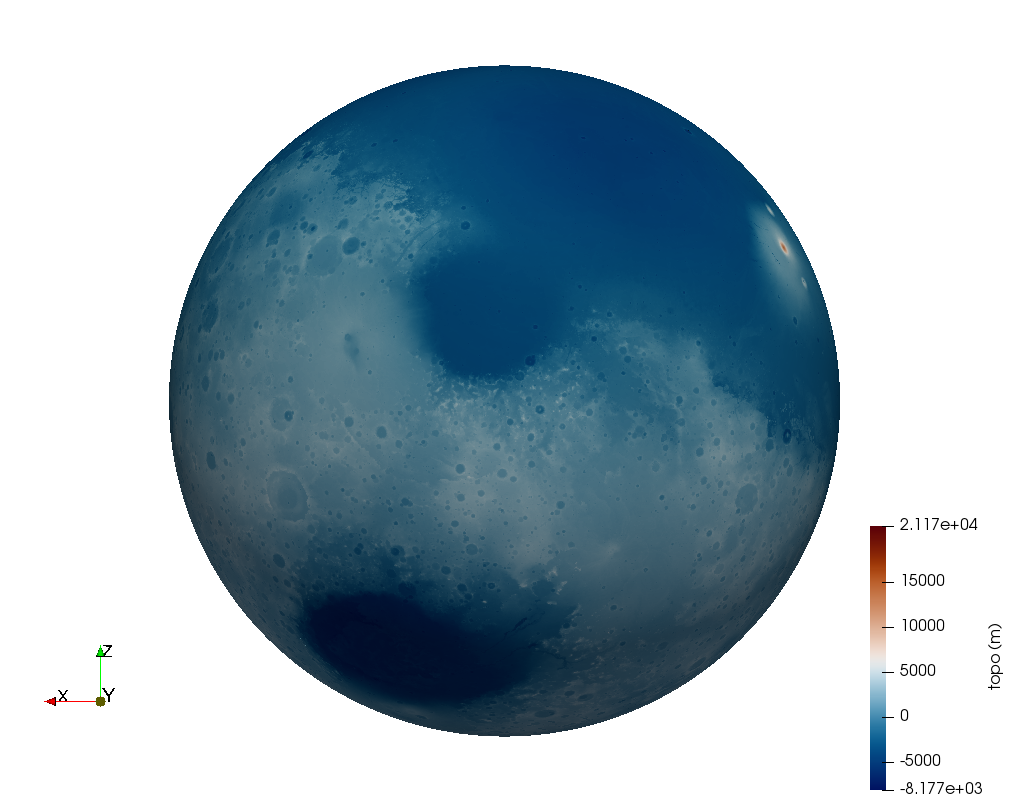
\includegraphics[width=5cm]{python_codes/fieldstone_100/images/topo3D_4}
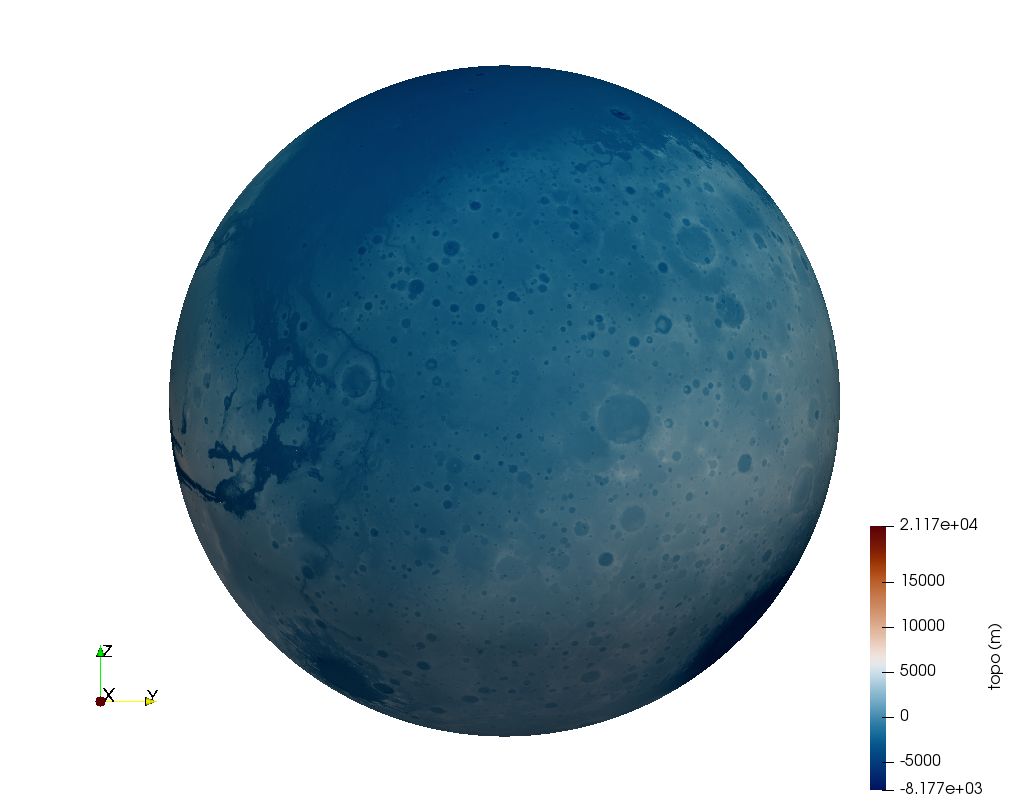
\includegraphics[width=5cm]{python_codes/fieldstone_100/images/topo3D_2}\\
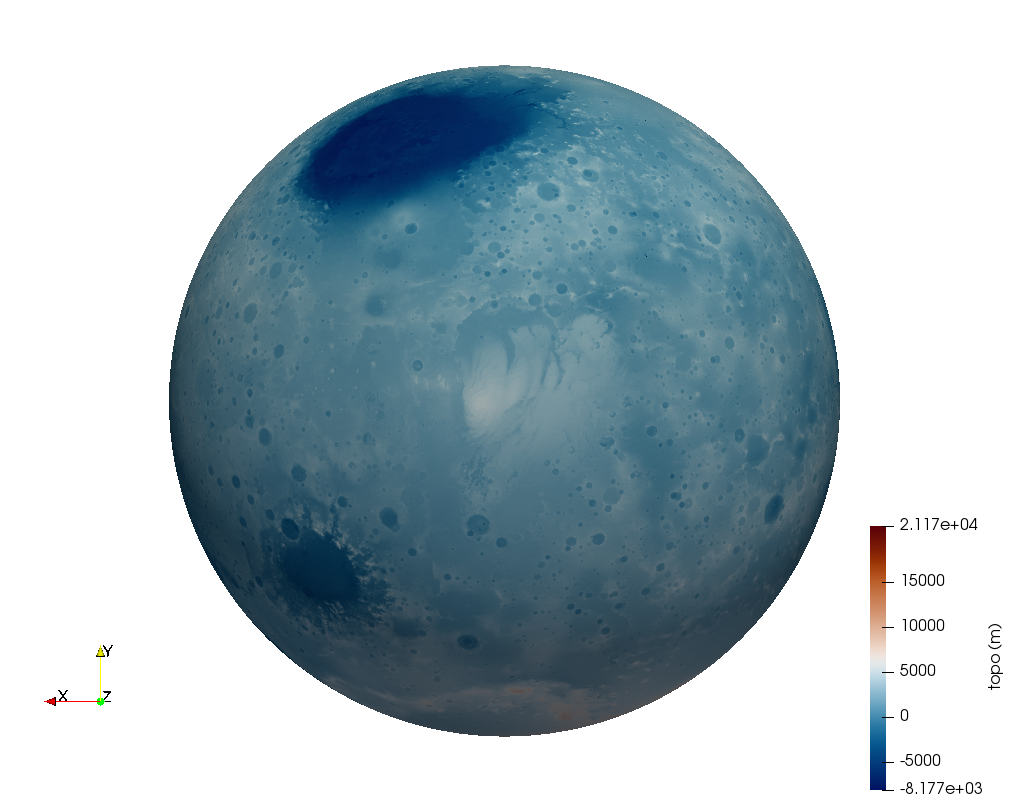
\includegraphics[width=5cm]{python_codes/fieldstone_100/images/topo3D_5}
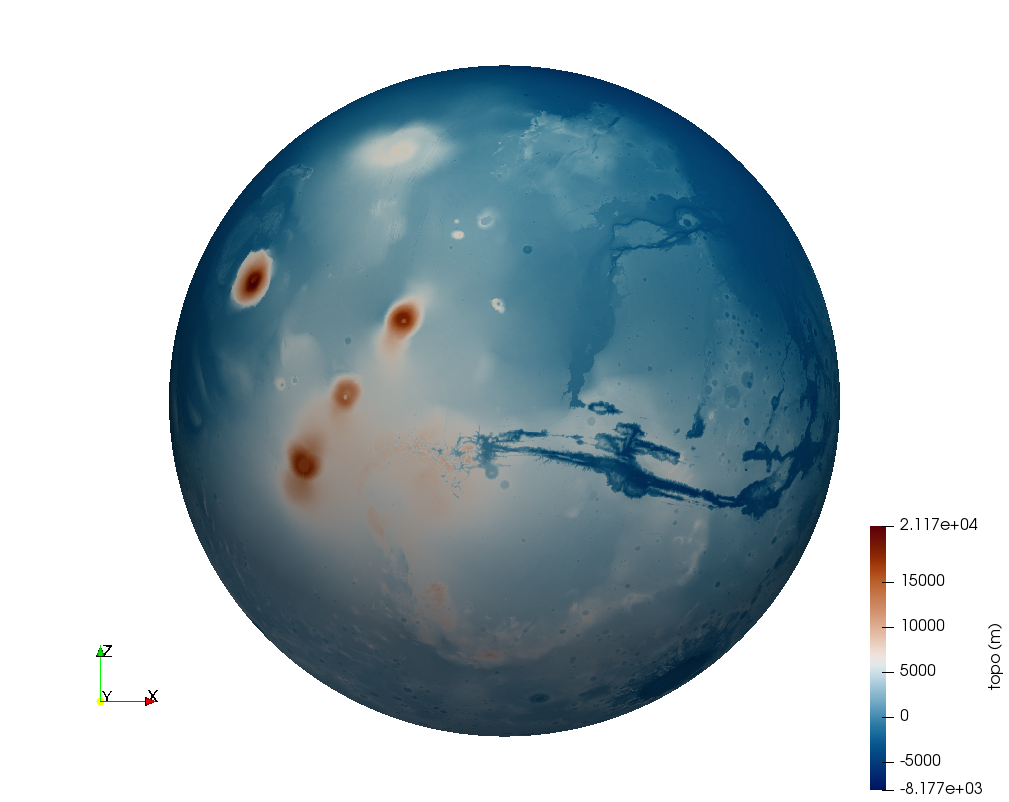
\includegraphics[width=5cm]{python_codes/fieldstone_100/images/topo3D_3}
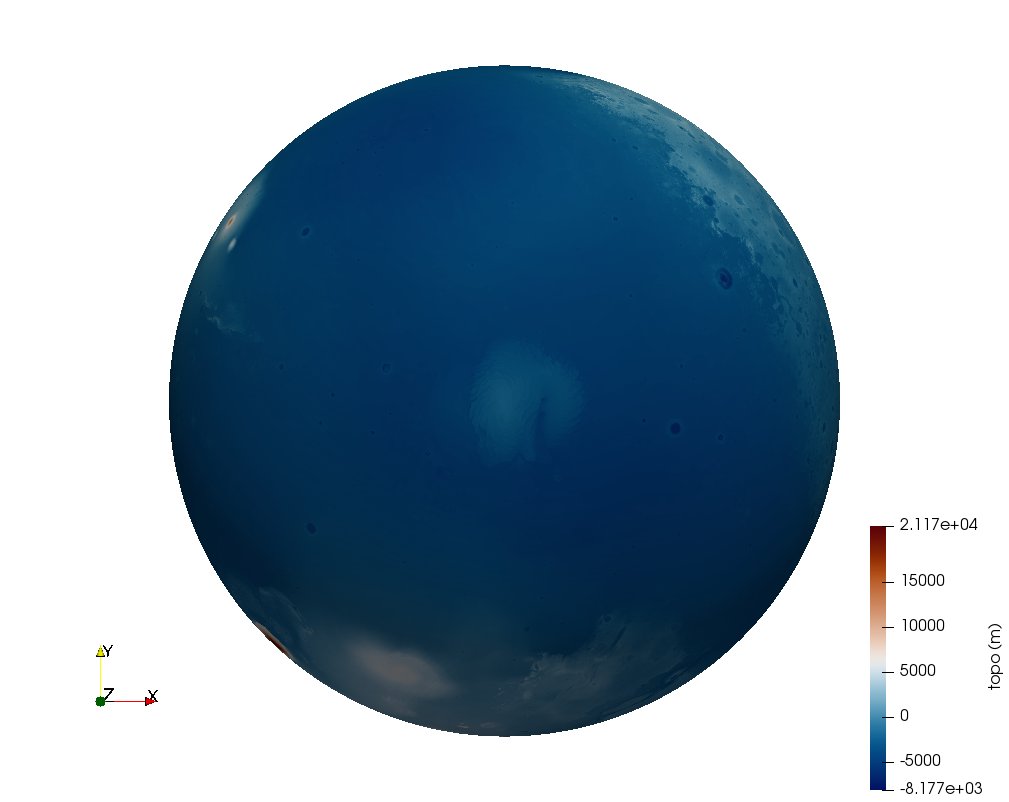
\includegraphics[width=5cm]{python_codes/fieldstone_100/images/topo3D_6}\\
{\captionfont Based on the 0.0625degree resolution file.}
\end{center}

